\sigla{GPS}{Sistema de Posicionamento Global}

\chapter{Fundamentação}
\label{fundamentacao}
Este capítulo aborda os principais fundamentos teóricos envolvidos na notificação oportuna de motoristas,
tema central deste trabalho. São apresentados conceitos sobre contexto, interrupção e notificação.
Ao final são apresentados alguns trabalhos correlatos.

\section{Contexto}
\label{contexto}
Em 1991, \cite{weiser1991computer} cunha o termo "Computação Ubíqua", que se refere ao caráter invisível da
integração de dispositivos computacionais diversos e da adaptação dos mesmos à necessidade do usuário no momento.
Um elemento bastante importante para a Computação Ubíqua é o estudo do contexto.

Contexto é definido por \cite{dey2001understanding} como "Qualquer informação que pode ser utilizada para
caracterizar a situação de entidades (ex: um usuário, lugar ou objeto) e que é considerada relevante para
a interação entre um usuário e uma aplicação, incluindo o próprio usuário e aplicação". Esta definição é
a mais utilizada na área e provavelmente a mais aceita. Alguns exemplos de elementos de contexto são
localização do usuário, ambiente, identidade do usuário e tempo \cite{ryan1999enhanced}.

Diversos sensores podem ser utilizados para determinar informações sobre o contexto do usuário. Alguns exemplos são
sensores de localização (GPS), sensores de luz e som, acelerômetro e giroscópio.

Informações de contexto são importantes para definir o estado atual do usuário e do ambiente onde ele está inserido,
mas somente isto é insuficiente. Para utilizar estas informações satisfatoriamente, é ideal que se construa um sistema
adaptativo e que supra as necessidades do usuário em tempo real utilizando as informações de contexto. Resumindo,
um sistema sensível ao contexto.

Sistemas sensíveis ao contexto são capazes de adaptar suas operações ao contexto atual, sem intervenção
explícita do usuário e têm como objetivo aumentar sua usabilidade e efetividade levando em conta elementos
de contexto \cite{baldauf2007survey}. Já \cite{abowd1999towards} define que um sistema é sensível ao contexto
se ele utiliza contexto para prover informações relevantes e/ou serviços para usuários, sendo que a relevância
depende das tarefas do usuário.

\section{Interrupção}
\label{interrupcao}



\subsection{Notificações e seu caráter interruptivo}
\label{notificacao}

\cite{iqbal2010notifications} define notificação como um sinal visual, audível ou táctil, gerado por uma aplicação
ou serviço e que passa informação para um usuário que está fora de seu foco de atenção. Em dispositivos móveis,
notificações geralmente são enviadas instantaneamente no momento em que ocorre alguma atividade que pode ser relevante
para o usuário quando a aplicação não está aberta, ex: Um email novo, uma mensagem de texto que acaba de chegar ou um
novo comentário em suas redes sociais. Em alguns casos o usuário toma ações imediatas após a chegada da notificação,
enquanto em outros ela é simplesmente ignorada. Essas ações dependem da importância da notificação e do contexto do
usuário \cite{sahami2014large}.

\begin{figure}[h]
\centering
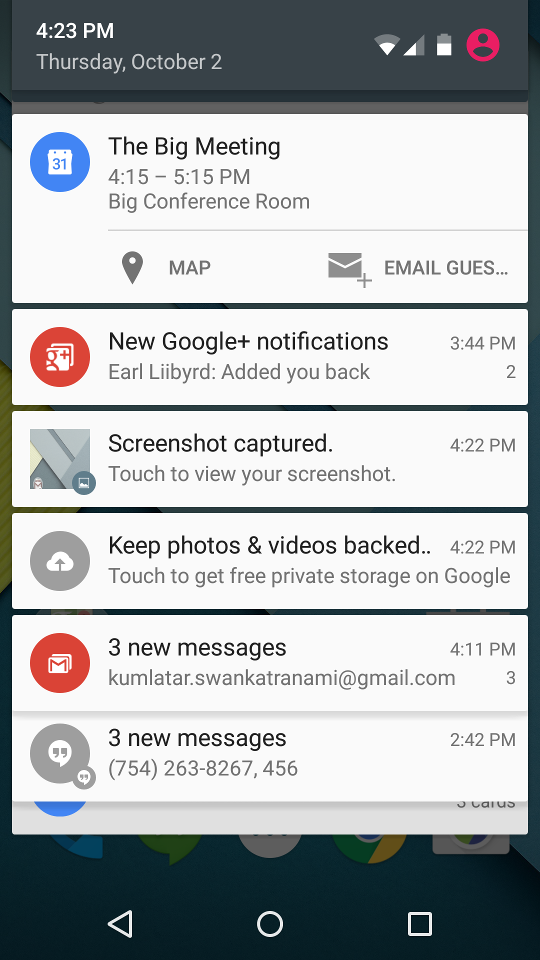
\includegraphics[width=0.3\textwidth]{imagens/notification_drawer.png}
\caption{Exemplo de notificações no Android \cite{notificationDrawer}}
\label{notification-drawer}
\end{figure}

\subsection{Interupção de Motoristas}
\label{interrupcao-motoristas}
